% Options for packages loaded elsewhere
\PassOptionsToPackage{unicode}{hyperref}
\PassOptionsToPackage{hyphens}{url}
%
\documentclass[
]{article}
\usepackage{lmodern}
\usepackage{amssymb,amsmath}
\usepackage{ifxetex,ifluatex}
\ifnum 0\ifxetex 1\fi\ifluatex 1\fi=0 % if pdftex
  \usepackage[T1]{fontenc}
  \usepackage[utf8]{inputenc}
  \usepackage{textcomp} % provide euro and other symbols
\else % if luatex or xetex
  \usepackage{unicode-math}
  \defaultfontfeatures{Scale=MatchLowercase}
  \defaultfontfeatures[\rmfamily]{Ligatures=TeX,Scale=1}
\fi
% Use upquote if available, for straight quotes in verbatim environments
\IfFileExists{upquote.sty}{\usepackage{upquote}}{}
\IfFileExists{microtype.sty}{% use microtype if available
  \usepackage[]{microtype}
  \UseMicrotypeSet[protrusion]{basicmath} % disable protrusion for tt fonts
}{}
\makeatletter
\@ifundefined{KOMAClassName}{% if non-KOMA class
  \IfFileExists{parskip.sty}{%
    \usepackage{parskip}
  }{% else
    \setlength{\parindent}{0pt}
    \setlength{\parskip}{6pt plus 2pt minus 1pt}}
}{% if KOMA class
  \KOMAoptions{parskip=half}}
\makeatother
\usepackage{xcolor}
\IfFileExists{xurl.sty}{\usepackage{xurl}}{} % add URL line breaks if available
\IfFileExists{bookmark.sty}{\usepackage{bookmark}}{\usepackage{hyperref}}
\hypersetup{
  hidelinks,
  pdfcreator={LaTeX via pandoc}}
\urlstyle{same} % disable monospaced font for URLs
\usepackage[margin=1in]{geometry}
\usepackage{color}
\usepackage{fancyvrb}
\newcommand{\VerbBar}{|}
\newcommand{\VERB}{\Verb[commandchars=\\\{\}]}
\DefineVerbatimEnvironment{Highlighting}{Verbatim}{commandchars=\\\{\}}
% Add ',fontsize=\small' for more characters per line
\usepackage{framed}
\definecolor{shadecolor}{RGB}{248,248,248}
\newenvironment{Shaded}{\begin{snugshade}}{\end{snugshade}}
\newcommand{\AlertTok}[1]{\textcolor[rgb]{0.94,0.16,0.16}{#1}}
\newcommand{\AnnotationTok}[1]{\textcolor[rgb]{0.56,0.35,0.01}{\textbf{\textit{#1}}}}
\newcommand{\AttributeTok}[1]{\textcolor[rgb]{0.77,0.63,0.00}{#1}}
\newcommand{\BaseNTok}[1]{\textcolor[rgb]{0.00,0.00,0.81}{#1}}
\newcommand{\BuiltInTok}[1]{#1}
\newcommand{\CharTok}[1]{\textcolor[rgb]{0.31,0.60,0.02}{#1}}
\newcommand{\CommentTok}[1]{\textcolor[rgb]{0.56,0.35,0.01}{\textit{#1}}}
\newcommand{\CommentVarTok}[1]{\textcolor[rgb]{0.56,0.35,0.01}{\textbf{\textit{#1}}}}
\newcommand{\ConstantTok}[1]{\textcolor[rgb]{0.00,0.00,0.00}{#1}}
\newcommand{\ControlFlowTok}[1]{\textcolor[rgb]{0.13,0.29,0.53}{\textbf{#1}}}
\newcommand{\DataTypeTok}[1]{\textcolor[rgb]{0.13,0.29,0.53}{#1}}
\newcommand{\DecValTok}[1]{\textcolor[rgb]{0.00,0.00,0.81}{#1}}
\newcommand{\DocumentationTok}[1]{\textcolor[rgb]{0.56,0.35,0.01}{\textbf{\textit{#1}}}}
\newcommand{\ErrorTok}[1]{\textcolor[rgb]{0.64,0.00,0.00}{\textbf{#1}}}
\newcommand{\ExtensionTok}[1]{#1}
\newcommand{\FloatTok}[1]{\textcolor[rgb]{0.00,0.00,0.81}{#1}}
\newcommand{\FunctionTok}[1]{\textcolor[rgb]{0.00,0.00,0.00}{#1}}
\newcommand{\ImportTok}[1]{#1}
\newcommand{\InformationTok}[1]{\textcolor[rgb]{0.56,0.35,0.01}{\textbf{\textit{#1}}}}
\newcommand{\KeywordTok}[1]{\textcolor[rgb]{0.13,0.29,0.53}{\textbf{#1}}}
\newcommand{\NormalTok}[1]{#1}
\newcommand{\OperatorTok}[1]{\textcolor[rgb]{0.81,0.36,0.00}{\textbf{#1}}}
\newcommand{\OtherTok}[1]{\textcolor[rgb]{0.56,0.35,0.01}{#1}}
\newcommand{\PreprocessorTok}[1]{\textcolor[rgb]{0.56,0.35,0.01}{\textit{#1}}}
\newcommand{\RegionMarkerTok}[1]{#1}
\newcommand{\SpecialCharTok}[1]{\textcolor[rgb]{0.00,0.00,0.00}{#1}}
\newcommand{\SpecialStringTok}[1]{\textcolor[rgb]{0.31,0.60,0.02}{#1}}
\newcommand{\StringTok}[1]{\textcolor[rgb]{0.31,0.60,0.02}{#1}}
\newcommand{\VariableTok}[1]{\textcolor[rgb]{0.00,0.00,0.00}{#1}}
\newcommand{\VerbatimStringTok}[1]{\textcolor[rgb]{0.31,0.60,0.02}{#1}}
\newcommand{\WarningTok}[1]{\textcolor[rgb]{0.56,0.35,0.01}{\textbf{\textit{#1}}}}
\usepackage{graphicx,grffile}
\makeatletter
\def\maxwidth{\ifdim\Gin@nat@width>\linewidth\linewidth\else\Gin@nat@width\fi}
\def\maxheight{\ifdim\Gin@nat@height>\textheight\textheight\else\Gin@nat@height\fi}
\makeatother
% Scale images if necessary, so that they will not overflow the page
% margins by default, and it is still possible to overwrite the defaults
% using explicit options in \includegraphics[width, height, ...]{}
\setkeys{Gin}{width=\maxwidth,height=\maxheight,keepaspectratio}
% Set default figure placement to htbp
\makeatletter
\def\fps@figure{htbp}
\makeatother
\setlength{\emergencystretch}{3em} % prevent overfull lines
\providecommand{\tightlist}{%
  \setlength{\itemsep}{0pt}\setlength{\parskip}{0pt}}
\setcounter{secnumdepth}{-\maxdimen} % remove section numbering

\author{}
\date{\vspace{-2.5em}}

\begin{document}

\hypertarget{musterloesung-aufgabe-2.3s-anova-mit-interaktion}{%
\subsection{Musterloesung Aufgabe 2.3S: ANOVA mit
Interaktion}\label{musterloesung-aufgabe-2.3s-anova-mit-interaktion}}

\begin{center}\rule{0.5\linewidth}{0.5pt}\end{center}

\begin{quote}
\textbf{Lese-Empfehlung} Kapitel 7 von
\href{https://mgimond.github.io/Stats-in-R/ANOVA.html}{Manny Gimond}
\end{quote}

\begin{quote}
Download \href{14_Statistik2/RFiles/solution_stat2.3s.R}{R-Skript}
\end{quote}

\begin{quote}
Download \href{14_Statistik2/RFiles/solution_stat2.3s.pdf}{PDF}
\end{quote}

\begin{center}\rule{0.5\linewidth}{0.5pt}\end{center}

\textbf{kommentierter Lösungsweg}

\begin{Shaded}
\begin{Highlighting}[]
\CommentTok{# klone den originaler Datensatz}
\NormalTok{df <-}\StringTok{ }\NormalTok{nova }

\CommentTok{# Daten vorbereiten}
\NormalTok{df }\OperatorTok\StringTok{ }\CommentTok{# schaut euch das Package "magrittr" an}
\StringTok{  }\CommentTok{# ersetze Local mit einem leeren String}
\StringTok{  }\KeywordTok{mutate}\NormalTok{(}\DataTypeTok{article_description =} \KeywordTok{str_replace}\NormalTok{(article_description, }\StringTok{"Local "}\NormalTok{, }\StringTok{""}\NormalTok{)) }\OperatorTok\StringTok{ }
\StringTok{  }\KeywordTok{filter}\NormalTok{(article_description }\OperatorTok{!=}\StringTok{ "Hot and Cold"}\NormalTok{) }\OperatorTok\StringTok{ }\CommentTok{# lasse Buffet Gerichte weg}
\StringTok{  }\KeywordTok{filter}\NormalTok{(member }\OperatorTok{!=}\StringTok{ "Spezialkarten"}\NormalTok{) }\OperatorTok\StringTok{ }\CommentTok{# Spezialkarten können vernachlässigt werden}
\StringTok{  }\CommentTok{#  fasse die zwei Menülinien "World & Favorite" zusammen}
\StringTok{  }\KeywordTok{mutate}\NormalTok{(}\DataTypeTok{article_description =} \KeywordTok{str_replace_all}\NormalTok{(article_description, }\StringTok{"Favorite|World"}\NormalTok{,}
                                               \StringTok{"Fav_World"}\NormalTok{))  }

\CommentTok{# gruppiere Daten nach Menülinie, Geschlecht und Hochschulzugehörigkeit}
\NormalTok{df }\OperatorTok
\StringTok{    }\KeywordTok{group_by}\NormalTok{(article_description, member, week) }\OperatorTok\StringTok{ }
\StringTok{    }\KeywordTok{summarise}\NormalTok{(}\DataTypeTok{tot_sold =} \KeywordTok{n}\NormalTok{()) }\OperatorTok
\StringTok{    }\KeywordTok{ungroup}\NormalTok{() }\OperatorTok\StringTok{ }
\StringTok{    }\KeywordTok{drop_na}\NormalTok{()  }\CommentTok{# lasst die unbekannten Menü-Inhalte weg}

\CommentTok{# überprüft die Voraussetzungen für eine ANOVA}
\CommentTok{# Schaut euch die Verteilungen der Mittelwerte der Responsevariable an}
\CommentTok{# Sind Mittelwerte nahe bei Null? Gäbe uns einen weiteren Hinweis auf }
\CommentTok{# eine spezielle Binomail-Verteilung (vgl. Statistik 4)}
\NormalTok{df }\OperatorTok\StringTok{ }
\StringTok{  }\KeywordTok{split}\NormalTok{(.}\OperatorTok{$}\NormalTok{article_description) }\OperatorTok\StringTok{ }\CommentTok{# teilt den Datensatz in 3 verschiedene Datensätze auf}
\StringTok{  }\CommentTok{# mit map können andere Funktionen auf den Datensatz angewendet werden }
\StringTok{  }\CommentTok{# (alternative Funktionen sind aggregate oder apply)}
\StringTok{  }\NormalTok{purrr}\OperatorTok{::}\KeywordTok{map}\NormalTok{(}\OperatorTok{~}\StringTok{ }\NormalTok{psych}\OperatorTok{::}\KeywordTok{describe}\NormalTok{(.}\OperatorTok{$}\NormalTok{tot_sold)) }
\end{Highlighting}
\end{Shaded}

\begin{verbatim}
## $Fav_World
##    vars  n   mean     sd median trimmed    mad min max range skew kurtosis   se
## X1    1 24 622.67 178.79  599.5   620.8 253.52 378 876   498 0.04    -1.88 36.5
## 
## $Kitchen
##    vars  n  mean    sd median trimmed   mad min max range skew kurtosis   se
## X1    1 24 128.5 22.21  124.5   128.2 23.72  79 187   108 0.27     0.43 4.53
\end{verbatim}

\begin{Shaded}
\begin{Highlighting}[]
\CommentTok{# visualisiere dir dein Model, was siehst du? }
\CommentTok{# sind möglicherweise gewiesse Voraussetzungen verletzt?}
\CommentTok{# Boxplot}
\KeywordTok{ggplot}\NormalTok{(df, }\KeywordTok{aes}\NormalTok{(}\DataTypeTok{x =} \KeywordTok{interaction}\NormalTok{(article_description, member), }\DataTypeTok{y=}\NormalTok{ tot_sold)) }\OperatorTok{+}\StringTok{ }
\StringTok{   }\CommentTok{# Achtung: Reihenfolge spielt hier eine Rolle!}
\StringTok{  }\KeywordTok{stat_boxplot}\NormalTok{(}\DataTypeTok{geom =} \StringTok{"errorbar"}\NormalTok{, }\DataTypeTok{width =} \FloatTok{0.25}\NormalTok{) }\OperatorTok{+}
\StringTok{  }\KeywordTok{geom_boxplot}\NormalTok{(}\DataTypeTok{fill=}\StringTok{"white"}\NormalTok{, }\DataTypeTok{color =} \StringTok{"black"}\NormalTok{, }\DataTypeTok{size =} \DecValTok{1}\NormalTok{, }\DataTypeTok{width =} \FloatTok{.5}\NormalTok{) }\OperatorTok{+}
\StringTok{  }\KeywordTok{labs}\NormalTok{(}\DataTypeTok{x =} \StringTok{"}\CharTok{\textbackslash{}n}\StringTok{Menülinie nach Hochschulzugehörigkeit"}\NormalTok{, }\DataTypeTok{y =} \StringTok{"Anzahl verkaufte Gerichte}\CharTok{\textbackslash{}n}\StringTok{"}\NormalTok{) }\OperatorTok{+}\StringTok{ }
\StringTok{  }\KeywordTok{scale_x_discrete}\NormalTok{(}\DataTypeTok{limits =} \KeywordTok{c}\NormalTok{(}\StringTok{"Fav_World.Mitarbeitende"}\NormalTok{, }\StringTok{"Kitchen.Mitarbeitende"}\NormalTok{,}
                              \StringTok{"Fav_World.Studierende"}\NormalTok{, }\StringTok{"Kitchen.Studierende"}\NormalTok{),}
                   \DataTypeTok{breaks =} \KeywordTok{c}\NormalTok{(}\StringTok{"Fav_World.Mitarbeitende"}\NormalTok{, }\StringTok{"Fav_World.Studierende"}\NormalTok{,}
                              \StringTok{"Kitchen.Mitarbeitende"}\NormalTok{,  }\StringTok{"Kitchen.Studierende"}\NormalTok{),}
                   \DataTypeTok{labels =} \KeywordTok{c}\NormalTok{(}\StringTok{"Fav_World}\CharTok{\textbackslash{}n}\StringTok{Mitarbeitende"}\NormalTok{, }\StringTok{"Fav_World}\CharTok{\textbackslash{}n}\StringTok{Studierende"}\NormalTok{,}
                              \StringTok{"Kitchen}\CharTok{\textbackslash{}n}\StringTok{Mitarbeitende"}\NormalTok{,  }\StringTok{"Kitchen}\CharTok{\textbackslash{}n}\StringTok{Studierende"}\NormalTok{)) }\OperatorTok{+}
\StringTok{  }\NormalTok{mytheme }\CommentTok{# wie sind die Voraussetzungen erfüllt?}
\end{Highlighting}
\end{Shaded}

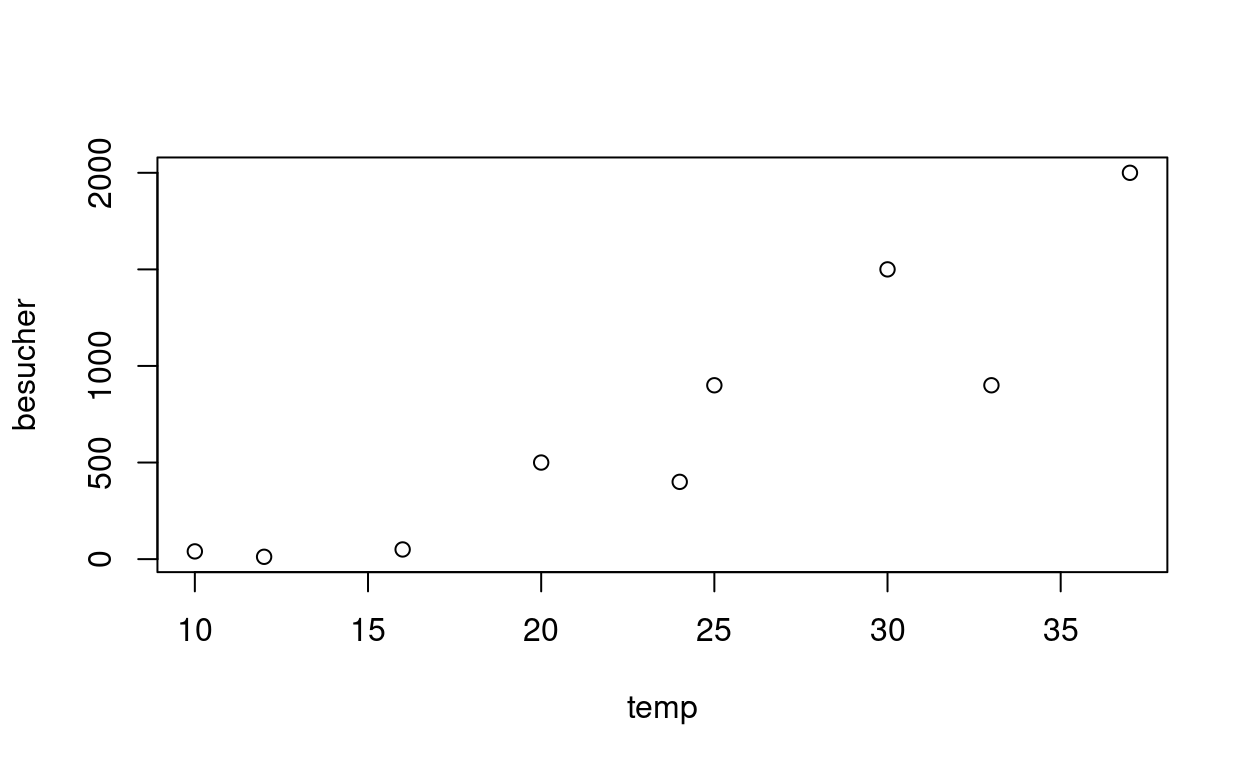
\includegraphics{solution_stat2.3s_files/figure-latex/unnamed-chunk-2-1.pdf}

\begin{Shaded}
\begin{Highlighting}[]
\CommentTok{# definiert das Modell (Skript Statistik 2)}
\NormalTok{model <-}\StringTok{ }\KeywordTok{aov}\NormalTok{(tot_sold }\OperatorTok{~}\StringTok{ }\NormalTok{article_description }\OperatorTok{*}\StringTok{ }\NormalTok{member, }\DataTypeTok{data =}\NormalTok{ df)}

\KeywordTok{summary.lm}\NormalTok{(model)}
\end{Highlighting}
\end{Shaded}

\begin{verbatim}
## 
## Call:
## aov(formula = tot_sold ~ article_description * member, data = df)
## 
## Residuals:
##    Min     1Q Median     3Q    Max 
## -91.00 -17.33   0.50  14.83  83.00 
## 
## Coefficients:
##                                              Estimate Std. Error t value
## (Intercept)                                   452.333      9.734   46.47
## article_descriptionKitchen                   -327.000     13.766  -23.75
## memberStudierende                             340.667     13.766   24.75
## article_descriptionKitchen:memberStudierende -334.333     19.469  -17.17
##                                              Pr(>|t|)    
## (Intercept)                                    <2e-16 ***
## article_descriptionKitchen                     <2e-16 ***
## memberStudierende                              <2e-16 ***
## article_descriptionKitchen:memberStudierende   <2e-16 ***
## ---
## Signif. codes:  0 '***' 0.001 '**' 0.01 '*' 0.05 '.' 0.1 ' ' 1
## 
## Residual standard error: 33.72 on 44 degrees of freedom
## Multiple R-squared:  0.9864, Adjusted R-squared:  0.9855 
## F-statistic:  1063 on 3 and 44 DF,  p-value: < 2.2e-16
\end{verbatim}

\begin{Shaded}
\begin{Highlighting}[]
\CommentTok{# überprüft die Modelvoraussetzungen (Statistik 2)}
\KeywordTok{par}\NormalTok{(}\DataTypeTok{mfrow =} \KeywordTok{c}\NormalTok{(}\DecValTok{2}\NormalTok{,}\DecValTok{2}\NormalTok{)) }\CommentTok{# alternativ gäbe es die ggfortify::autoplot(model) funktion}
\KeywordTok{plot}\NormalTok{(model)}
\end{Highlighting}
\end{Shaded}

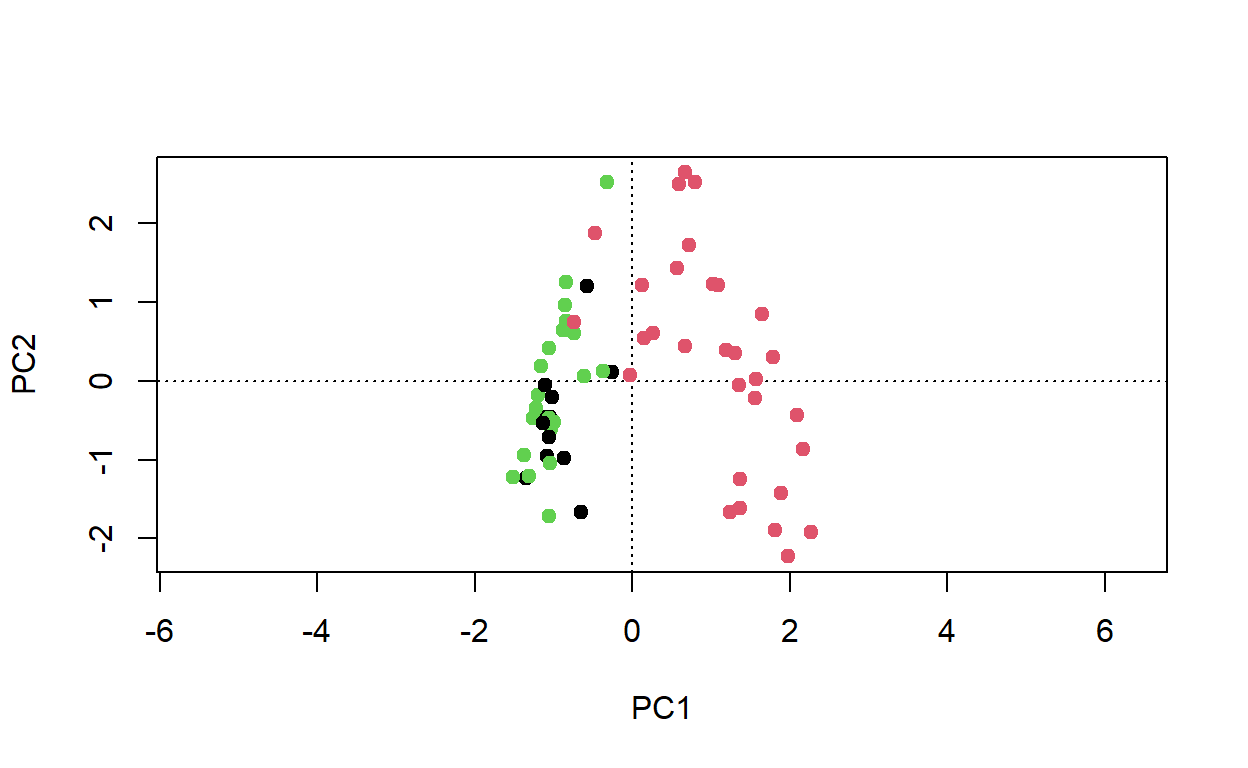
\includegraphics{solution_stat2.3s_files/figure-latex/unnamed-chunk-2-2.pdf}

{ \textbf{Fazit}: Die Inspektion des Modells zeigt kleinere Verletzungen
bei der Normalverteilung der Residuen (Q-Q Plot). Aufgrund keiner
starken Verbesserung durch eine Transformation der Responsevariable,
entscheide ich mich für eine ANOVA ohne log-tranformierten
Responsevariablen (AV).}

\begin{Shaded}
\begin{Highlighting}[]
\CommentTok{# sieht aus, als ob die Voraussetzungen für eine Anova nur geringfügig verletzt sind}
\CommentTok{# mögliche alternativen: }
\CommentTok{# 1. log-transformation um die grossen werte zu minimieren (nur möglich, wenn }
\CommentTok{# keine 0 enthalten sind und die Mittelwerte weit von 0 entfernt sind }
\CommentTok{# => bei Zähldaten ist dies leider nicht immer gegeben)}
\CommentTok{# 2. nicht parametrische Test z.B. Welch-Test, da hohe Varianzheterogenität }
\CommentTok{# zwischen den Residuen}


\CommentTok{#1) log-transformation}
\NormalTok{model_log <-}\StringTok{ }\KeywordTok{aov}\NormalTok{(}\KeywordTok{log10}\NormalTok{(tot_sold) }\OperatorTok{~}\StringTok{ }\NormalTok{article_description }\OperatorTok{*}\StringTok{ }\NormalTok{member, }\DataTypeTok{data =}\NormalTok{ df)}

\KeywordTok{summary.lm}\NormalTok{(model_log) }\CommentTok{# interaktion ist nun nicht mehr signifikant: vgl. }
\end{Highlighting}
\end{Shaded}

\begin{verbatim}
## 
## Call:
## aov(formula = log10(tot_sold) ~ article_description * member, 
##     data = df)
## 
## Residuals:
##       Min        1Q    Median        3Q       Max 
## -0.191372 -0.025043  0.003191  0.037604  0.182842 
## 
## Coefficients:
##                                              Estimate Std. Error t value
## (Intercept)                                   2.65417    0.01696 156.533
## article_descriptionKitchen                   -0.56517    0.02398 -23.569
## memberStudierende                             0.24438    0.02398  10.191
## article_descriptionKitchen:memberStudierende -0.21726    0.03391  -6.407
##                                              Pr(>|t|)    
## (Intercept)                                   < 2e-16 ***
## article_descriptionKitchen                    < 2e-16 ***
## memberStudierende                            3.71e-13 ***
## article_descriptionKitchen:memberStudierende 8.51e-08 ***
## ---
## Signif. codes:  0 '***' 0.001 '**' 0.01 '*' 0.05 '.' 0.1 ' ' 1
## 
## Residual standard error: 0.05874 on 44 degrees of freedom
## Multiple R-squared:  0.9745, Adjusted R-squared:  0.9728 
## F-statistic: 561.4 on 3 and 44 DF,  p-value: < 2.2e-16
\end{verbatim}

\begin{Shaded}
\begin{Highlighting}[]
\CommentTok{# nochmals euren Boxplot zu beginn, machen diese Koeffizienten sinn?}

\CommentTok{# überprüft die Modelvoraussetzungen (vgl. Skript Statistik 2)}
\CommentTok{# bringt aber keine wesentliche Verbesserung, daher bleibe ich bei den }
\CommentTok{# untranfromierten Daten}
\KeywordTok{par}\NormalTok{(}\DataTypeTok{mfrow =} \KeywordTok{c}\NormalTok{(}\DecValTok{2}\NormalTok{,}\DecValTok{2}\NormalTok{))}
\KeywordTok{plot}\NormalTok{(model_log)}
\end{Highlighting}
\end{Shaded}

\begin{verbatim}
## hat values (leverages) are all = 0.08333333
##  and there are no factor predictors; no plot no. 5
\end{verbatim}

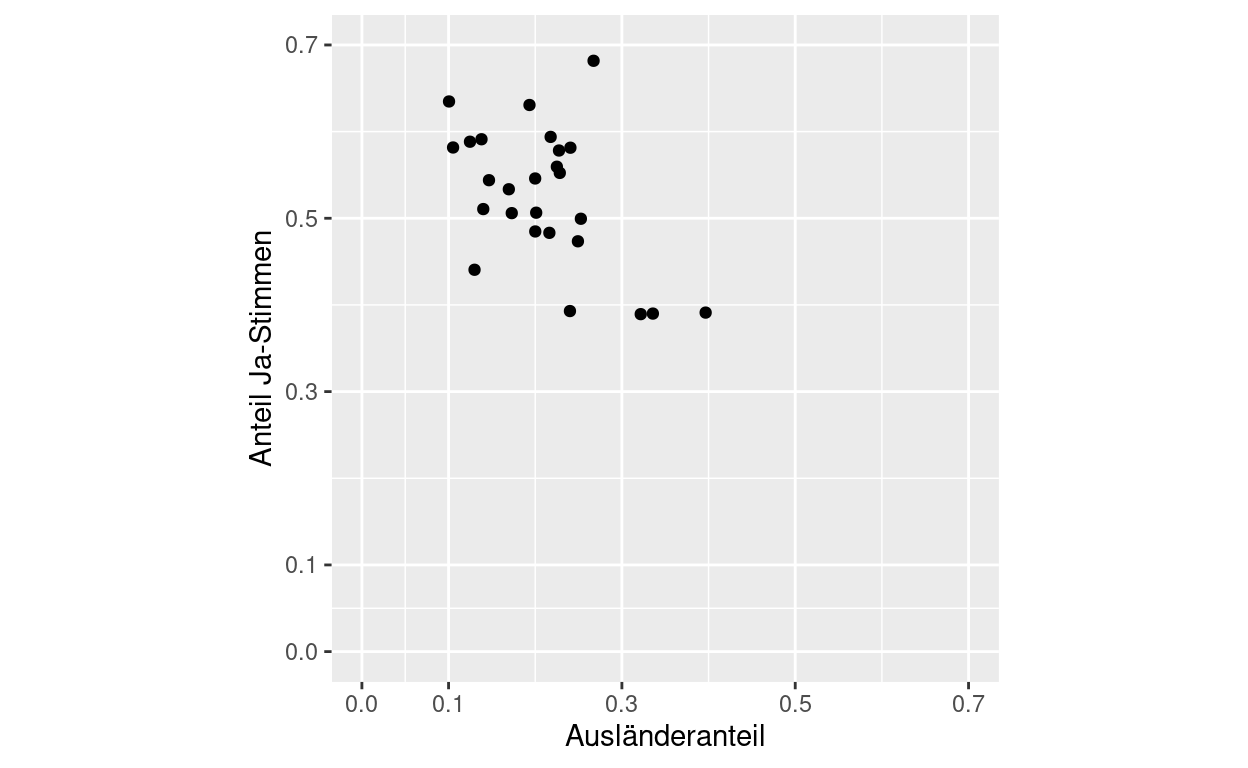
\includegraphics{solution_stat2.3s_files/figure-latex/unnamed-chunk-3-1.pdf}

\begin{Shaded}
\begin{Highlighting}[]
\CommentTok{# post-hov Vergleiche}
\KeywordTok{TukeyHSD}\NormalTok{(model)}
\end{Highlighting}
\end{Shaded}

\begin{verbatim}
##   Tukey multiple comparisons of means
##     95% family-wise confidence level
## 
## Fit: aov(formula = tot_sold ~ article_description * member, data = df)
## 
## $article_description
##                        diff      lwr       upr p adj
## Kitchen-Fav_World -494.1667 -513.785 -474.5484     0
## 
## $member
##                            diff      lwr      upr p adj
## Studierende-Mitarbeitende 173.5 153.8817 193.1183     0
## 
## $`article_description:member`
##                                                      diff        lwr        upr
## Kitchen:Mitarbeitende-Fav_World:Mitarbeitende -327.000000 -363.75650 -290.24350
## Fav_World:Studierende-Fav_World:Mitarbeitende  340.666667  303.91017  377.42317
## Kitchen:Studierende-Fav_World:Mitarbeitende   -320.666667 -357.42317 -283.91017
## Fav_World:Studierende-Kitchen:Mitarbeitende    667.666667  630.91017  704.42317
## Kitchen:Studierende-Kitchen:Mitarbeitende        6.333333  -30.42317   43.08983
## Kitchen:Studierende-Fav_World:Studierende     -661.333333 -698.08983 -624.57683
##                                                   p adj
## Kitchen:Mitarbeitende-Fav_World:Mitarbeitende 0.0000000
## Fav_World:Studierende-Fav_World:Mitarbeitende 0.0000000
## Kitchen:Studierende-Fav_World:Mitarbeitende   0.0000000
## Fav_World:Studierende-Kitchen:Mitarbeitende   0.0000000
## Kitchen:Studierende-Kitchen:Mitarbeitende     0.9672944
## Kitchen:Studierende-Fav_World:Studierende     0.0000000
\end{verbatim}

\begin{center}\rule{0.5\linewidth}{0.5pt}\end{center}

\textbf{Methode}

Ziel war es die Unterschiede zwischen den preisgünstigeren und teureren
Menülinien und der Hochschulzugehörigkeit herauszufinden: Hierfür wurde
eine ANOVA mit Interaktion gerechnet, da wir eine (quasi)-metrische
Responsevariable und zwei Prädiktorvariablen (Menülinie und
Hochschulzugehörigkeit) haben. Die Voraussetzungen für eine ANOVA waren
im ersten Model nicht stark verletzt, lediglich die Normalverteilung der
Residuen: Deshalb habe wurde auf eine log-Transformation der
Responsevariable verzichtet. Anschliessend wurden noch post-hoc
Einzelvergleiche nach Tukey durchgeführt.

\begin{center}\rule{0.5\linewidth}{0.5pt}\end{center}

\textbf{Ergebnisse}

Die wöchentlichen Verkaufszahlen der Menülinien unterscheiden sich nach
Hochschulzugehörigkeit signifikant (F(3,44) = 561.42, p \textless{}
.001). Inhaltich bedeutet dies, dass Studierende signifikant häufiger
die preisgünstigere Menülinie ``Favorite \& World'' als Mitarbeitende
kaufen. Entgegen der Annahme gibt es aber keine signifikanten
Unterschiede zwischen Studierende und Mitarbeitende bei dem Kauf der
teureren Menülinie ``Kitchen''. Über die möglichen Gründe können nur
spekuliert werden, hierfür bedarf es weiteren Analysen z.B. mit dem
Prädiktor ``Menüinhalt''.

\begin{figure}
\centering
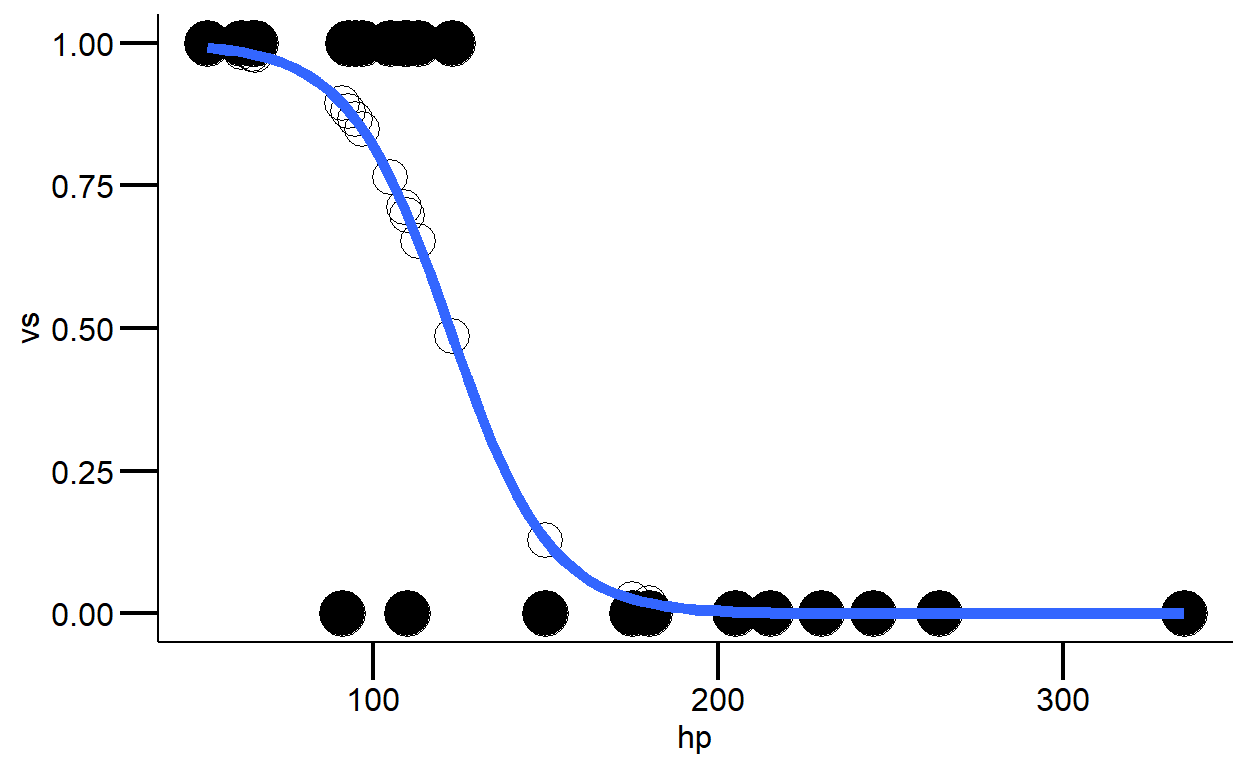
\includegraphics{solution_stat2.3s_files/figure-latex/unnamed-chunk-4-1.pdf}
\caption{Box-Whisker-Plots der wöchentlichen Verkaufszahlen pro
Menü-Inhalte. Kleinbuchstaben bezeichnen homogene Gruppen auf \emph{p}
\textless{} .05 nach Tukeys post-hoc-Test.}
\end{figure}

\end{document}
